%%%%%%%%%%%%%%%%%%%%%%%%%%%%%%%%%%%%%%%%%%%%%%%%%%%%%%%%%%%%%%%%%%%%
%% I, the copyright holder of this work, release this work into the
%% public domain. This applies worldwide. In some countries this may
%% not be legally possible; if so: I grant anyone the right to use
%% this work for any purpose, without any conditions, unless such
%% conditions are required by law.
%%%%%%%%%%%%%%%%%%%%%%%%%%%%%%%%%%%%%%%%%%%%%%%%%%%%%%%%%%%%%%%%%%%%

\documentclass{beamer}
\usetheme[faculty=ped]{fibeamer}
\usepackage[utf8]{inputenc}
\usepackage{pscyr}
\usepackage{ragged2e}
\usepackage[english,russian]{babel}        %% typeset as follows:
%%
%%   \begin{otherlanguage}{czech}   ... \end{otherlanguage}
%%   \begin{otherlanguage}{slovak}  ... \end{otherlanguage}
%%
%% These macros specify information about the presentation
\title{Развитие матричного представления обобщенных графовых структур в задачах описания и анализа Больших Данных} %% that will be typeset on the
\subtitle{Алексей Приньков} %% title page.
\author{д.ф.-м.н, профессор, С.Л. Блюмин sabl@lipetsk.ru, студент, А.С. Приньков, aprinkov@gmail.com, кафедра прикладной математики}
%% These additional packages are used within the document:
\usepackage{ragged2e}  % `\justifying` text
\usepackage{booktabs}  % Tables
\usepackage{tabularx}
\usepackage{tikz}

\usepackage{multirow} %объединение строк в таблицах
\usepackage{tabularx}
\usetikzlibrary{matrix}
\usetikzlibrary{calc, shapes, backgrounds}
\usepackage{amsmath, amssymb}
\usepackage{url}       % `\url`s
\usepackage{listings}  % Code listings
\frenchspacing
\begin{document}
	% \frame{\maketitle}

	\AtBeginSection[]{% Print an outline at the beginning of sections
		\begin{frame}<beamer>
			\frametitle{Содержание раздела \thesection}
			\tableofcontents[currentsection]
		\end{frame}}

	\begin{darkframes}
		\begin{frame}
			\begin{tikzpicture}[overlay,remember picture]
					\node[anchor=north west,xshift=0,yshift=0pt]
						at (current page.north west) {
							\includegraphics[width=0.12\paperwidth]{resources/stu}

							\includegraphics[width=0.86\paperwidth]{resources/graphhpclogo}
						};
				\end{tikzpicture}%
							\vspace*{1.4cm}

			\usebeamercolor[fg]{frametitle}%
			\usebeamerfont{frametitle}%
			\centering
				Развитие матричного представления обобщенных графовых структур в задачах описания и анализа Больших Данных\\
				...........................................
			\usebeamercolor[fg]{subtitle}%
			\usebeamerfont{subtitle}%
			\\Приньков Алексей
					\vfill
			\usebeamerfont{author}%
			\usebeamercolor[fg]{author}
			\centering  
				д.ф.-м.н., профессор Блюмин С.Л., sabl@lipetsk.ru, +7(910)-350-44-40
				\\студент Приньков А.С., aprinkov@gmail.com, +7(910)-250-55-40
				\\\vspace{0.1cm}\tiny{Кафедра прикладной математики, Липецкий государственный технический университет}
	\end{frame}
		\begin{frame}{}
			\begin{block}{Цель работы}
			\centering
				Целью данной ВКР является развитие методов графоструктурного моделирования и применение разработанных методов и инструментов к задачам анализа и описания больших данных. В частности, для решения задачи обработки данных процесса холодного проката разнотолщинной стали стана 2030 с целью выявления причин вибраций
			\end{block}
		\end{frame}
		\section{Графоструктурное моделирование}
		\subsection{Графы и их обобщение}
		\begin{frame}{Графы}
			\begin{block}{Определение функции $B$}
				\centering
				$B(V,n) =[V \rightarrow 2^V ] ^n,$\\ где $[S]^n = \{X \mid X \subseteq S \wedge |X| = n\}$.
			\end{block}
% https://math.stackexchange.com/questions/678753/is-there-a-commonly-accepted-notation-for-k-subsets
			\begin{block}{Формальное определение графа}
				\centering
				\alert{Граф} -- это $\langle V, E \rangle$,  где $E \subseteq B(V,2)$.
			\end{block}
			\centering
			\includegraphics[scale=0.1]{resources/graph}
		\end{frame}
		\begin{frame}[label=lists]{Обобщенные графовые структуры}
						\begin{block}{Гиперграф}
							\centering
							\alert{Гиперграф} определен как $\langle V, HE\rangle$, где $HE \subseteq \bigcup \limits_{i=1}^{n}B(V,i)$.
						\end{block}
						\begin{block}{Гиперсеть}
							\centering
							\alert{Гиперсеть} -- это пара, состоящая из множества гиперребер и множества отображений между ними $HN = \langle \{WS_i\}, \{\Phi_i\}\rangle$, где $WS_i$ -- гиперребро, а $\Phi_i: WS_i \to WS_{i-1}$.
						\end{block}
						\begin{columns}[onlytextwidth]
						\column{.5\textwidth}
						 \centering
							\includegraphics[scale=0.1]{resources/hypergraph}
						\column{.5\textwidth}
						 \centering
							\includegraphics[scale=0.1]{resources/hypernetwork}
						\end{columns}
		\end{frame}
		

	\begin{frame}[label=lists]{Обобщенные графовые структуры}
			\begin{block}{Метаграф}
				\centering
				\alert{Метаграф} -- это $MG=\langle V, ME \rangle$, где $V$ -- множество вершин, $ME$ -- множество \alert{метаребер} и $ME\subseteq B( \bigcup \limits_{i=1}^{n}B(V, i),2)$.
						 
			\end{block}

		 \begin{block}{Эквивалентное определние метаграфа}
			 \centering
			 $MG=\langle V, MV, ME \rangle,$ где множество \alert{метавершин} $MV \subseteq \bigcup \limits_{i=1}^{n}B(V, i)$, а $ME\subseteq B(MV,2)$. 
			\end{block}
	
			\centering
				\includegraphics[scale=0.1]{resources/mg}
	\end{frame}

	\begin{frame}[label=lists]{Обобщенные графовые структуры}
	 	\begin{block}{Итергиперграфы}\centering \small{
	 		$V$--некоторое множество, $f:V \to 2^V$.
		\\$f(V,0) = V, f(V,1) = f(V), f(V,2) = f(f(V)), f(V,p) = f(f(V, p-1))$,
	 		где $p$ - показатель итерации и $e(f(V,p))=p, e(f(V,p)) = e(f(V,p-1))+1$.

	 		Если  $|V|=n, |E|=m |f(V,p)| \leq m \leq |f(V,p+1)|$,\\ то $e(E)$ дробный показатель итерации.}
	 	\end{block}
	 		Для графа показатель итерации равен $\frac{n-m}{2^n-n}$.\\Для гиперграфа и метаграфа $\frac{n-m}{2^n-n}, \frac{2^n-m}{2^{2^n}-2^n}$ соответственно.
	 		
	 		\justifying
	 		Класс итергиперграфов охватывает все графовые структуры при варьировании степени итерации.
	\end{frame}

		\subsection{Особенности метаграфов}

	\begin{frame}[label=lists]{Особенности метаграфов}
	\centering
	 	Характерной особенностью метаграфа является то, что он обобщает приведенные графовые структуры и что в нём реализованы \alert{два вида смежности} вершин.\\ Причем одна из смежностей должна однозначно определять связи между вершинами.


	 	\vspace*{0.7cm}
			\begin{columns}[onlytextwidth]
			\begin{column}{0.48\columnwidth}
			\centering
			\textbf{Метавершинная}
			% \smallskip
				\begin{itemize}
					\item \scriptsize{$G\langle V, E \rangle \cong MG\langle V, MV, ME \rangle,$ где $ME =\varnothing$, а $MV \subseteq B(V, 2) = E$ }
					\item \scriptsize{$HG\langle V, HE \rangle \cong MG\langle V, MV, ME \rangle,$ где $ME =\varnothing$, а $MV \subseteq \bigcup \limits_{i=1}^{n}B(V, i) = HE$}
					\item \scriptsize{$HN \langle WS, \Phi \rangle \cong MG\langle V, MV, ME \rangle = \Big\langle V, \{WS_i\},  \big\langle ..., \langle WS_i , WS_{i-1}\rangle, ...  \big\rangle \Big\rangle$}
				\end{itemize}
			\end{column}

			\begin{column}{0.48\columnwidth}
			\centering
			\textbf{Метареберная}
			% \smallskip
				\begin{itemize}
					\item \scriptsize{$G\langle V, E \rangle \cong MG\langle V, MV, ME \rangle,$ где $MV \subseteq \bigcup \limits_{i=1}^{n}B(V, i), ME \subseteq B(MV,2)$}
					\item \scriptsize{$HG\langle V, HE \rangle \cong MG\langle V, MV, ME \rangle,$ где  $MV \subseteq \bigcup \limits_{i=1}^{n}B(V, i), ME \subseteq B(MV,2)$}
					\item \scriptsize{$HN \langle WS, \Phi \rangle \cong MG\langle V, MV, ME \rangle = \Big\langle V, \{WS_i\},  \big\langle ..., \langle WS_i , WS_{i-1}\rangle, ...  \big\rangle \Big\rangle$}
				\end{itemize}
			\end{column}
			\end{columns}
	\end{frame}

	\begin{frame}[label=lists]{Особенности метаграфов}
	\centering 
		Вторая функция смежности может использоваться для ...\smallskip

			\begin{tabular}{|p{0.48\textwidth}|p{0.48\textwidth}|} \hline
					... рассмотрения \alert{связей между связями}. Например, между двумя ребрами:
						&
					... кластеризации вершин. Например, для \alert{кластеризации} вершин по признаку совместной смежности другой вершине: \\
					\hline
					\centering 
					\includegraphics[scale=0.1]{resources/rtr} & \includegraphics[scale=0.1]{resources/rtc} \\ \hline
			\end{tabular}
	\end{frame}

	% \begin{frame}[label=lists]{Особенности метаграфов}
	% \hspace*{-1cm}
	% 	\begin{tabular}{|p{3cm}|p{8cm}|}
	% 	\hline
	% 		Какая смежность соотв. <<обычной>> связи & Граф / Гиперграф / Метаграф \\ \hline
	% 		Метавершинная & \includegraphics[scale=0.1]{resources/rtr}  \\ \hline
	% 	\end{tabular}
	% \end{frame}

	\begin{frame}[label=lists]{Особенности метаграфов}
		\centering
		Метаграф не только обобщает приведенные структуры, но и достаточен по отношению к более абстрактным структурам в задачах моделирования, т.к. ...
		\definecolor{sthlmBlue}{RGB}{0,110,191}
		\definecolor{sthlmLightPurple}{RGB}{93,35,125}
		\setbeamercolor{boxsthlmBlue}{bg=sthlmBlue,fg=white}
		\setbeamercolor{boxsthlmPurple}{bg=sthlmLightPurple,fg=white}


		\vspace*{0.7cm}
			\begin{columns}[onlytextwidth]
				\begin{column}{0.48\columnwidth}
					\begin{beamercolorbox}[wd=\linewidth,ht=10ex,dp=3ex]{boxsthlmBlue}
					\centering
						... связи могут быть между связями произвольного уровня.
					\end{beamercolorbox}
				% \centering
				% \begin{block}{
				% }\
				% \end{block}
				\end{column}

				\begin{column}{0.48\columnwidth}
				\centering

				\begin{beamercolorbox}[wd=\linewidth,ht=10ex,dp=3ex]{boxsthlmPurple}
					\centering
						... кластеризация вершин может быть многокритериальной.
					\end{beamercolorbox}
				\end{column}
			\end{columns}
	\end{frame}

	\subsection{Матричное представление}
		\begin{frame}[label=simmonshall]{Матричное представление}
		\centering
			Графовые структуры удобно представлять с помощью матриц. Для такого представления наиболее популярны матрицы \alert{инцидентности} ($I$), \alert{смежности} ($A$), \alert{валентности} ($D$) и \alert{лапласиан} ($L$), которые связаны равенством 
			\\$I \cdot I^{\tau} = L = D \pm A.$

				
		\end{frame}

		\begin{frame}{Матричное представление}
		\centering

			Также \alert{любую графовую структуру} можно представить в матричном виде с помощью графа Кёнига:

			\includegraphics[scale=0.22]{resources/kenig}
		\end{frame}

		\begin{frame}{Матричное представление}
			\centering
			\alert{Матрица смежности по Басу:} \\$a_{ij}=\bigcup \limits_k(\alpha_{ij})_k, $
			где			\vspace*{-0.3cm}

			\begin{equation*}
			(\alpha_{ij})_k = 
			 \begin{cases}
			   \langle mu_k\{v_i\}, mv_k\{v_j\},\langle me_k \rangle \rangle, & \text{ если } v_i \in mu_k \wedge v_j \in mv_k ;\\
			   \varnothing, & \text{ иначе.}
			 \end{cases}
			\end{equation*} 
			\vspace*{-0.5cm}
			\centering
			
				\includegraphics[scale=0.23]{resources/basuadj}
		\end{frame}

		\begin{frame}{Матричное представление}
		 \centering
		 На основе слайда 6 выводится связь между матричными представлениями разных графовых структур как частных случаев итергиперграфов. Например, для метаграфа матрица инцидентности определяется как
			$$I(V,ME) = I(V,E) \cdot I(MV, ME).$$
		\end{frame}

		\begin{frame}{Матричное представление}
			\centering
			Взаимосвязь $L(V,ME)$ и $I(V,E)$, $I(MV,ME)$: $L(V,ME) = I(V,ME)\cdot I(MV,ME)=$
				 $$ \scriptsize =
					\left(
					\begin{array}{c|c|c}
					 \begin{array}{ccc}
					    l_{1,1} & ...& 0\\
					    \vdots& \ddots &\vdots \\
					    0&... & \ddots
					  \end{array}
					   & I(V, MV) & 0 \\
					\hline
					(I(V,MV))^\tau &  \begin{array}{ccc}
					    \ddots & ...& 0\\
					    \vdots& \ddots &\vdots \\
					    0&... & \ddots
					  \end{array} & I(MV, ME)  \\
					\hline
					0 & (I(MV,ME))^\tau &  \begin{array}{ccc}
					   \ddots & ...& 0\\
					    \vdots& \ddots &\vdots \\
					    0&... & l_{|V|+|MV|+|ME|,|V|+|MV|+|ME|}
					  \end{array}
					\end{array}
					\right),$$ где  $l_{i,i}=\sum\limits_{k=1}^{|V+E|} |l_{i,k}|=\sum\limits_{k=1}^{|V+E|} |l_{k,i}|.$
		\end{frame}

		\begin{frame}[label=simmonshall]{Матричное представление}
		\frametitle{Какое из представлений выбрать?!}
		\justifying
			Выбор матричного представления должен осуществляться в зависимости от \alert{постановки} задач, \alert{наличия реализованных алгоритмов} для данного представления, а также возможности \alert{корректной интерпретации} промежуточных и конечного результата.
			\vspace{0.5cm}
			\centering
			\includegraphics[width=0.9\paperwidth]{resources/algebra}

			% \includegraphics[width=0.75\paperwidth]{resources/algebra2}

		\end{frame}

	\begin{frame}{Пути реализации матричного представления }
	\centering
			\begin{columns}[onlytextwidth]
				\begin{column}{0.3\columnwidth}
				\centering
					\alert{Алгоритмический}
					
				\end{column}

				\begin{column}{0.3\columnwidth}
				\centering
					$+$
				\end{column}

				\begin{column}{0.3\columnwidth}
				\centering
					\alert{Алгебраический}
				\end{column}
			\end{columns}

			\begin{itemize}
				\item Базовые операции линейной алгебры;
				\item алгоритмические операции;
				\item логика и алгебра высказываний;
				\item идемпотентные полукольца.	
			\end{itemize}
		\end{frame}

		\begin{frame}{Преимущества матричного подхода}
			\begin{itemize}
				\justifying
				\item Возможность оптимизации вычислений с использованием архитектуры параллельного программирования и распределенного хранения данных;
				\item строгая алгебраическая формализация;
				\item применимость средств линейной алгебры и основанных на ней методов прикладной математики;
				\item вариативность представления в зависимости от условий задачи.
			\end{itemize}	
		
		\end{frame}


	\subsection{Ремоделирование и его мотивация}
		\begin{frame}[label=math]{Ремоделирование и его мотивация}
		\centering
			\alert{Математическое ремоделирование} -- это подход на основе перехода от математических или имитационных моделей одного или различных типов к моделям некоторого одного класса. 
			\\\alert{Суть подхода} -- приведение исходных моделей к единой форме, пригодной или удобной для дальнейшего анализа и исследования.
			\\\alert{Особенностью подхода} является то, что начальной информацией является некоторая математическая или имитационная модель, а не информация об объекте или процессе моделирования. 
		\end{frame}


		\begin{frame}[label=math]{Ремоделирование и его мотивация}
			\frametitle{Результаты применения гиперграфов}
			
				\begin{itemize}
					\centering
					\item \alert{Сложные системы}
					\item \alert{Машинное обучение}
					\item \alert{Реализация неинтуитивных связей}
					\item \alert{Относительная простота интерпретации}
				\end{itemize}
		\begin{flushleft}
		\begin{thebibliography}{9}
		\scriptsize{
				\item[1] S. Tan, Z. Guan, D. Cai, X. Qin, J. Bu, and C. Chen. Mapping users across networks by manifold alignment on hypergraph. In AAAI, 2014. 

				\item[2] Huang, J. Scalable Hypergraph Learning and Processing [Text] / Huang J. Zhang R.,  Xu Yu J. // Data Mining (ICDM), 2015 IEEE International Conference on --- Atlantic City, NJ, USA, 14-17 Nov. 2015. 
			
				\item[3]  Zhou, D. Learning with Hypergraphs: Clustering, Classification, and Embedding [Text] / D. Zhou, J. Huang, B. Schölkopf // AINPS 19, 2007 --- p. 1601-1608.
				\item[4]  Blyumin, S.L. Interval Cyclic Hypergraphs for Modeling of Transportation Systems [Text] / S.L. Blyumin, A.V. Galkin, D.L. Prikhodko, P.V. Saraev, A.S Sysoev // ICTTE, 2014. ---  Belgrade , Serbia --- pp 157-163. }
		\end{thebibliography}
		\end{flushleft}

   	
	\end{frame}

	% \begin{frame}[label=lists]{Краткие итоги}
	% 	Здесь показать почему именно метаграфы
	% \end{frame}


	% \subsection{Эмерджентность} не знаю куда

		\subsection{Список литературы}
		\begin{frame}[label=bibliography]{Список литературы}
			\begin{thebibliography}{9}
					\justifying
				\small{
				\item[1] Емеличев, В.А. Лекции по теории графов [Текст] / В.А. Емеличев, О.И. Мельников, В.И. Сарванов, Р.И. Тышкевич. --- М.: Наука, 1990. --- 384 с.

				\item[2] Basu, A. Metagraphs and Their Applications [Text] / A. Basu, R. Blanning. --- NY: Springer, 2007. --- 172 р.	


				\item[3] Блюмин, С.Л. Итергиперграфы: расширенный класс графовых моделей больших систем [Текст]  / С.Л. Блюмин //  Труды конференции <<Теория активных систем-2011>> (ТАС) в рамках Международной научно-практической мультиконференции <<Управление большими системами>> (УБС-2011). --- Москва: ИПУ РАН, 2011. --- Т.1. --- С. 11-15.

				\item[4] Блюмин, С.Л. Графоструктурное моделирование. Метаграфы и их матрицы [Текст] / С.Л. Блюмин // Вестник ЛГТУ. --- 2015. --- №~1(23). --- С. 7-13.				
}

				
			\end{thebibliography}
		\end{frame}

		\begin{frame}[label=bibliography]{Список литературы}
			\begin{thebibliography}{9}

			\small{

				\item[5] Блюмин, С.Л. Оргипергиперграфы: матрицы инцидентности и лапласианы [Текст] / С.Л. Блюмин // Вестник ЛГТУ. --- 2013. --- №~1(21). --- С. 15-27.

				\item[6] Приньков, А.С. Графоструктурное ремоделирование метаграфами сложных систем на примере московского метрополитена [Текст] : HTCS'2017 : мат-лы XII междунар. науч.-практ. конф., 25-27 октября 2017 г. --- С. 125-129.

				\item[7] Приньков, А.С. Разработка программного обеспечения для графоструктурного ремоделирования сложных систем [Текст] : HTCS'2017 : мат-лы XII междунар. науч.-практ. конф., 25-27 октября 2017 г.. --- С. 65-69.

				\item[8] Etsuji, T. The worst-case time complexity for generating all maximal cliques and computational experiments / T. Etsuji, T. Akira, T. Haruhisa // Theoretical Computer Science, volume 363, issue 1, 2006 --- pp 28-42.


			}

			\end{thebibliography}
		\end{frame}


		%----------------------------------------
\section{Описание и анализ Больших Данных}
\subsection{Алгоритм преобразования графа в метаграф}
		\begin{frame}{Алгоритм преобразования графа в метаграф}
			\begin{enumerate}
				\item Запишем граф в виде матрицы инцидентности $I(V,E)$.
				\item Если матрица $I(V,E)=\mathbb{O}$, то алгоритм завершен.
				\item Находим строку в $I(V,E)$ с максимальным количеством единиц (вершину с максимальной валентностью).
				\item Добавляем метаребро в $I(V,ME)$, содержащее в одной метавершине эту вершину, а в другой метавершине вершины, смежные с данной.
				\item Обнуляем в $I(V,ME)$ найденную строку и столбцы, значения которых в этой строке равны единице.
				\item Переходим к пункту 2.
			\end{enumerate}
		\end{frame}

		\begin{frame}[fragile]	
\frametitle{Пример использования алгоритма}
\textit{Пример.} Дан граф $G = \langle V, E\rangle  = \big\langle \{ v_1, v_2, v_3, v_4, v_5 \},  \{ v_1, v_2 \},  \{v_1, v_3\},\{v_2, $\\$v_3\}, \{v_2, v_4\}, \{v_3, v_4\}, \{v_4, v_5\} \big\rangle$. Необходимо преобразовать его в метаграф, иными словами, построить изоморфный ему метаграф.

Матрица инцидентности графа $G(V,E)$ и матрица инцидентности метаграфа $MG(V, ME)$ в начале вычислений равны
$$I(V,E) =
\left(
\begin{array}{cccccc}
1 & 1 & 0 & 0 & 0 & 0 \\
1 & 0 & 1 & 1 & 0 & 0 \\
0 & 1 & 1 & 0 & 1 & 0 \\
0 & 0 & 0 & 1 & 1 & 1 \\
0 & 0 & 0 & 0 & 0 & 1 \\ 
\end{array}
\right),
I(V,ME) = ().
$$
\end{frame}

\begin{frame}[fragile]
\frametitle{Пример использования алгоритма}
Первая итерация.
$$
I(V,E) =
\begin{tikzpicture}[baseline=-0.5ex]
     \matrix (mat) [%
       matrix of nodes,
       left delimiter={(},right delimiter={)}
     ]
      {%
        1 & 1 & 0 & 0 & 0 & 0 \\
		1 & 0 & 1 & 1 & 0 & 0 \\
		0 & 1 & 1 & 0 & 1 & 0 \\
		0 & 0 & 0 & 1 & 1 & 1 \\
		0 & 0 & 0 & 0 & 0 & 1 \\ 
      };
    % do the strike out thing
		\draw[white] (mat-2-1.west)  -- (mat-2-6.east);
		\draw[white] (mat-1-1.north) -- (mat-5-1.south);
		\draw[white] (mat-1-3.north) -- (mat-5-3.south);
		\draw[white] (mat-1-4.north) -- (mat-5-4.south);
\end{tikzpicture}
= \left(
\begin{array}{cccccc}
	0 & 1 & 0 & 0 & 0 & 0 \\
	0 & 0 & 0 & 0 & 0 & 0 \\
	0 & 1 & 0 & 0 & 1 & 0 \\
	0 & 0 & 0 & 0 & 1 & 1 \\
	0 & 0 & 0 & 0 & 0 & 1 \\ 
\end{array}
\right),
$$$$
I(V,ME) 
= \left(
\begin{array}{c}
1 \\
-1 \\
1 \\
1 \\
0 \\
\end{array}
\right).
$$
\end{frame}

\begin{frame}[fragile]
\frametitle{Пример использования алгоритма}

Вторая итерация.
$$I(V,E) =
\begin{tikzpicture}[baseline=-0.5ex]
     \matrix (mat) [%
       matrix of nodes,
       left delimiter={(},right delimiter={)}
     ]
      {%
        0 & 1 & 0 & 0 & 0 & 0 \\
		0 & 0 & 0 & 0 & 0 & 0 \\
		0 & 1 & 0 & 0 & 1 & 0 \\
		0 & 0 & 0 & 0 & 1 & 1 \\
		0 & 0 & 0 & 0 & 0 & 1 \\ 
      };
    % do the strike out thing
		\draw[white] (mat-3-1.west)  -- (mat-3-6.east);
		\draw[white] (mat-1-2.north) -- (mat-5-2.south);
		\draw[white] (mat-1-5.north) -- (mat-5-5.south);


\end{tikzpicture}
= \left(
\begin{array}{cccccc}
	0 & 0 & 0 & 0 & 0 & 0 \\
	0 & 0 & 0 & 0 & 0 & 0 \\
	0 & 0 & 0 & 0 & 0 & 0 \\
	0 & 0 & 0 & 0 & 0 & 1 \\
	0 & 0 & 0 & 0 & 0 & 1 \\ 
\end{array}
\right),
$$
$$
I(V,ME) = 
\left(
\begin{array}{cc}
1 & 1\\
-1 & 0\\
1 &  -1\\
1 & 1\\
0 &  0\\
\end{array}
\right).
$$
\end{frame}

\begin{frame}[fragile]
\frametitle{Пример использования алгоритма}
Третья итерация.
$$I(V,E) =
\begin{tikzpicture}[baseline=-0.5ex]
     \matrix (mat) [%
       matrix of nodes,
       left delimiter={(},right delimiter={)}
     ]
      {%
		0 & 0 & 0 & 0 & 0 & 0 \\
		0 & 0 & 0 & 0 & 0 & 0 \\
		0 & 0 & 0 & 0 & 0 & 0 \\
		0 & 0 & 0 & 0 & 0 & 1 \\
		0 & 0 & 0 & 0 & 0 & 1 \\ 
      };
    % do the strike out thing
		\draw[white] (mat-5-1.west)  -- (mat-5-6.east);
		\draw[white] (mat-1-6.north) -- (mat-5-6.south);


\end{tikzpicture}
= \left(
\begin{array}{cccccc}
	0 & 0 & 0 & 0 & 0 & 0 \\
	0 & 0 & 0 & 0 & 0 & 0 \\
	0 & 0 & 0 & 0 & 0 & 0 \\
	0 & 0 & 0 & 0 & 0 & 0 \\
	0 & 0 & 0 & 0 & 0 & 0 \\ 
\end{array}
\right) = \mathbb{O},
$$
$$
I(V,ME) = 
\left(
\begin{array}{ccc}
1 & 1 & 0 \\
-1 & 0 & 0 \\
1 &  -1& 0 \\
1 & 1 & 1 \\
0 &  0 & -1 \\
\end{array}
\right).
$$
\end{frame}

		\subsection{Сложные системы}
		\begin{frame}{Сложные системы}
			\begin{block}{Определение сложной системы}
			\centering
				Сложная система -- система, состоящая из множества взаимодействующих подсистем, вследствие чего сложная система приобретает новые свойства, характерные для неё как для целостной структуры, которые отсутствуют не только у каждой подсистемы в частности, но и у суммы подсистем.
			\end{block}
		\end{frame}

		\begin{frame}[label=math]{Сложные системы -- эмерджентные свойства}
		\centering
			Примеры систем с эмерджентными свойствами:
			\begin{itemize}
				\item живые организмы;
				\item текст на естественном языке;
				\item интеллект;
				\item социальная сеть;
				\item производственное предприятие.
			\end{itemize}



			Эмерджентные свойства \alert{не восходят к количеству}.
			Источником эмерджентных свойств является структура системы: при различной структуре у систем, образуемых из одних и тех же элементов, возникают разные свойства и особенности.

			\includegraphics[width=0.17\paperwidth]{resources/glider}

		\end{frame}

		\begin{frame}{Сложные системы -- иллюстрация}
			\centering
			\begin{columns}[onlytextwidth]
				\begin{column}{0.6\columnwidth}
					\centering
					 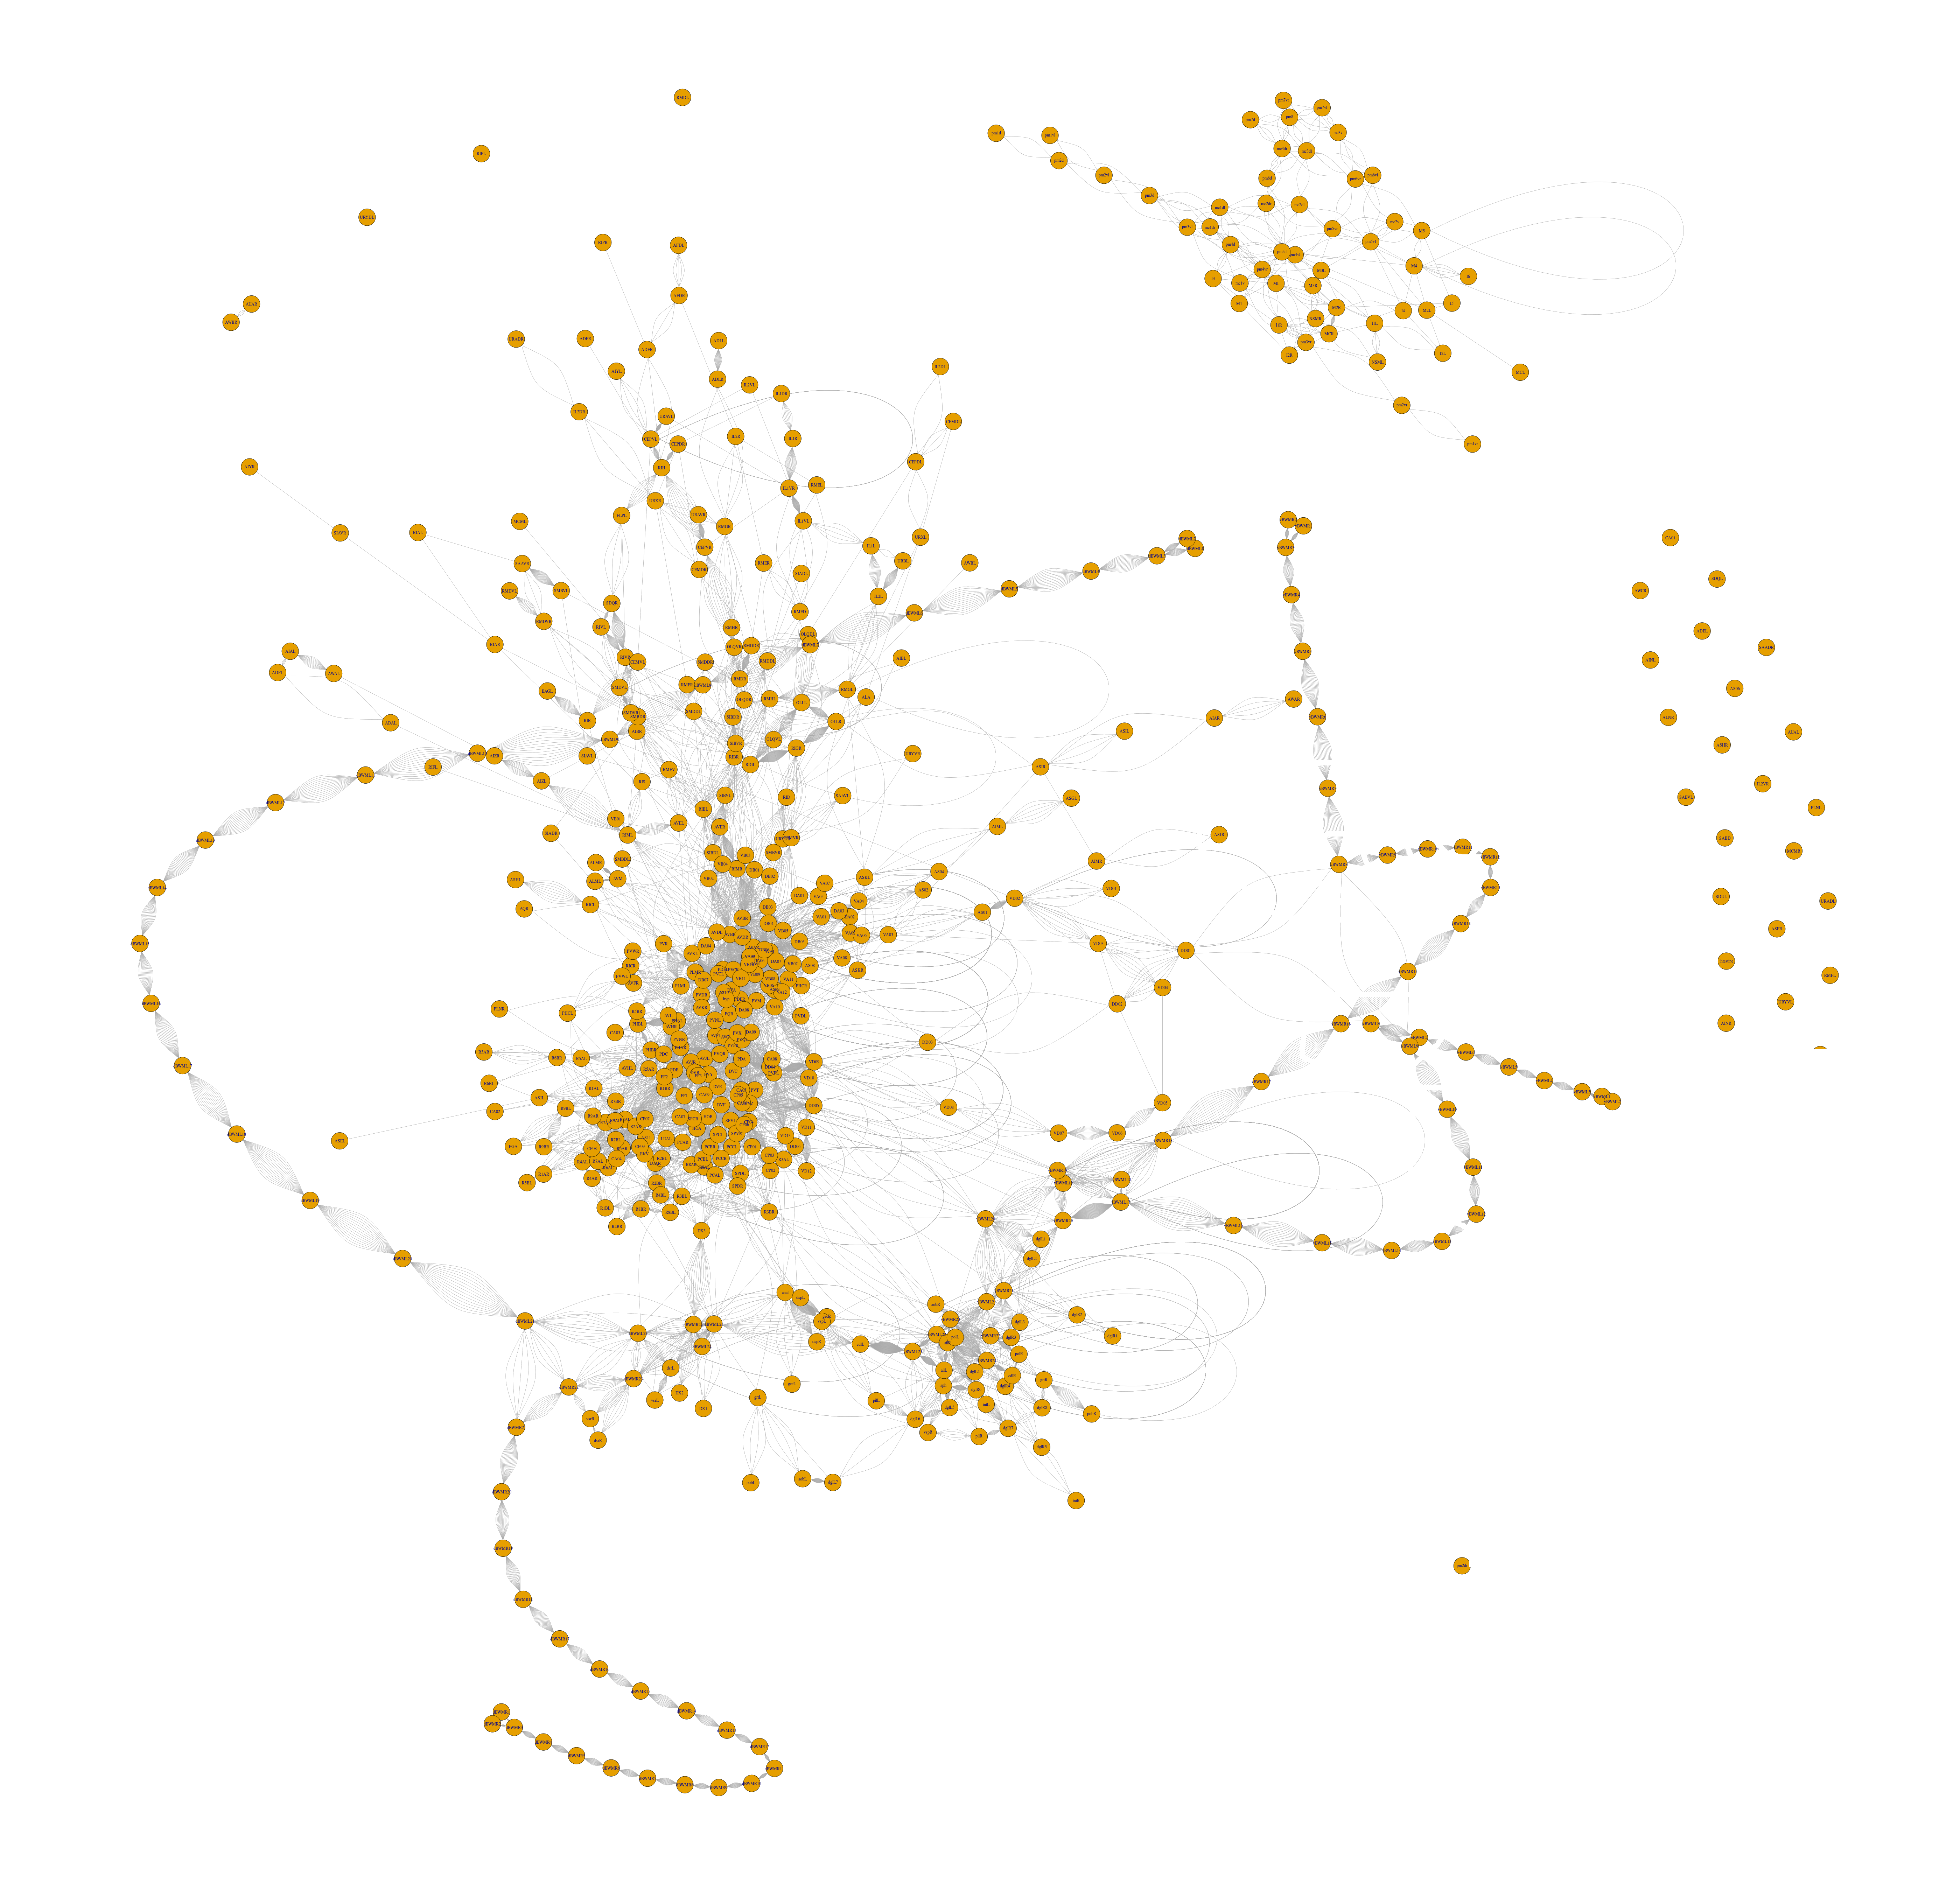
\includegraphics[width=0.58\paperwidth]{resources/complex}

				\end{column}

				\begin{column}{0.38\columnwidth}
					\centering
					\vspace*{4cm}
					\begin{itemize}
						\item \alert{Распределенные} вычисления;
						\item \alert{не нужно} искать клики (!NP);
						\item относительная \alert{простота} интерпретации.
					\end{itemize}	

				\end{column}
			\end{columns}
		\end{frame}
	
		\subsection{ИИС и ГИИС}
		\begin{frame}{ИИС и ГИИС}

			\begin{block}{}
			\centering
				Применение графоструктурного подхода к решению задач больших данных можно условно разделить на два вида -- это непосредственно моделирование исходных данных графовыми структурами и моделирование информационных систем (ИС), с помощью которых решаются эти задачи.

			\end{block}
		\end{frame}

		\begin{frame}{Реализация ГИИС}
			\centering
			Программную реализацию простейших видов ГИИС можно найти в библиотеке машинного обучения sklearn.
			\begin{columns}[onlytextwidth]
				\begin{column}{0.48\columnwidth}
					\centering

					Pipeline\\
					\includegraphics[width=0.23\paperwidth]{resources/linear}

				\end{column}

				\begin{column}{0.48\columnwidth}
					\centering

					FeatureUnions\\
					\includegraphics[width=0.4\paperwidth]{resources/parallel}
				\end{column}
			\end{columns}

		\end{frame}
		
		\subsection{Практические примеры}

		\begin{frame}{Практические примеры-классификация текста}
		\centering
		Исходные данные
			\begin{tabular}{|c|c|p{3cm}|c|}
			\hline
			PhraseId & SentenceId & Phrase & Sentiment \\ \hline
			1 & 1 & A series of escapades demonstrating the adage ... & 1 \\ \hline
			2 & 1 &demonstrating the adage & 2 \\ \hline
			 ... & ... & ...  & ... \\ \hline
			156060 & 8544 & avuncular chortles & 3 \\\hline  
			\end{tabular}
		Источник: https://www.kaggle.com/c/sentiment-analysis-on-movie-reviews
		\end{frame}

		\begin{frame}{Практические примеры-классификация текста}
		\centering
			Лексический анализатор
			$$x' = g(x), g:\mathbb{L} \to \mathbb{R}^{n_1}.$$
			Отображение-трансформатор
		 	$$x_2' = h(x_1'), h: \mathbb{R}^{n_1} \to \mathbb{R}^{n_2}.$$
		 	Процесс предварительной обработки данных
		 	$$h_n(...(h_1(g_1(x)))), g_1 : \mathbb{L} \to \mathbb{R}^{n_1}, h_i:\mathbb{R}^{n_{i}} \to \mathbb{R}^{n_{i+1}}. $$

		\end{frame}

		\begin{frame}{Практические примеры-классификация текста}
		\centering
			Для параллельной обработки данных необходимо использовать метаграфовую структуру ГИИС:

$$x_g' = Gx =
\left(
\begin{array}{c}
g_1 \\
g_2\\
\vdots \\
g_{n-1}\\ 
g_{n}
\end{array}
\right)^{\tau}
\left(
\begin{array}{ccccc}
x & 0 & ... &  0 & 0 \\
0 & x & ... & 0 & 0 \\
\vdots & \vdots & \vdots & \vdots & \vdots \\
0 & 0 & ... & x & 0 \\
0 & 0 & ... & 0 & x
\end{array}
\right)  = 
\left(
\begin{array}{c}
g_1(x) \\
g_2(x)\\
\vdots \\
g_{n-1}(x)\\ 
g_n(x)
\end{array}
\right)^{\tau}.
$$ 
После чего получится разреженная матрица, которую необходимо преобразовать в векторную форму
$$x_{g}' = m_g(x'), m_g : \mathbb{R}^{n_1 \times n} \to \mathbb{R}^{n'},$$
		\end{frame}
		\begin{frame}{Практические примеры-классификация текста}
			к которой можно применить отображения-трансформаторы либо последовательно
$$h_n(...(h_1(g_1(x_{g})))), g_1 : \mathbb{L} \to \mathbb{R}^{n_1}, h_i:\mathbb{R}^{n_{i}} \to \mathbb{R}^{n_{i+1}},$$
либо параллельно
$$\tiny{x'_h  =
\left(
\begin{array}{c}
h_1 \\
h_2\\
\vdots \\
h_{n-1}\\ 
h_{n}
\end{array}
\right)^{\tau}
\cdot
m_g
\left(\left(
\begin{array}{c}
g_1 \\
g_2\\
\vdots \\
g_{n-1}\\ 
g_{n}
\end{array}
\right)^{\tau}
\cdot\left(
\begin{array}{ccccc}
x & 0 & ... &  0 & 0 \\
0 & x & ... & 0 & 0 \\
\vdots & \vdots & \vdots & \vdots & \vdots \\
0 & 0 & ... & x & 0 \\
0 & 0 & ... & 0 & x
\end{array}
\right) \right)  = 
\left(
\begin{array}{c}
h_1(x'_g) \\
h_2(x'_g)\\
\vdots \\
h_{n-1}(x'_g)\\ 
h_n(x'_g)
\end{array}
\right)^{\tau}.}
$$ 
В случае параллельного применения трансформаторов

$$x_{h}' = m_h(x'), m_h : \mathbb{R}^{n_2 \times n} \to \mathbb{R}^{n'}.$$
		\end{frame}

		\begin{frame}{Практические примеры-классификация текста}
			Построим ГИИС для предварительной обработки данных, состоящую из трех метавершин. $MG = \Big\langle \{h_1, h_2, h_3, g_1, g_2, g_3$\\$, g_4\}, \big \langle \langle \{h_2, h_3\}, \{g_1, g_2, g_3,g_4\} \rangle, \langle \{h_1\},\{h_2, h_3, g_1, g_2, g_3, g_4$\\$\} \rangle \big \rangle\Big\rangle$, где $g_1,g_2, g_3, g_4$ -- лексические анализаторы, а $h_1, h_2, h_3$ -- трансформаторы.
			\begin{itemize}
				\item $g_1$ = tfidf (N-граммы по словам);
				\item $g_2$ = tfidf (N-граммы по буквам);
				\item $g_3$, $g_4$ -- <<счетчики>>;
			\end{itemize}	

			$h_1,h_2,h_3$ -- трансформаторы для масштабирования входных векторов до единичной нормы с использованием $l_1,l_2, \max$ нормы соотвественно.

			Результат: $84\%$ train, $67\%$ test.
		\end{frame}


	
		\subsection{Список литературы}
		\begin{frame}[label=bibliography]{Список литературы}
			\begin{thebibliography}{9}
					\justifying
				\small{
					\item[1] Блюмин, С.Л. Графоструктурные тенденции развития ИИС: применение гиперграфов, метаграфов, итерграфов и их матричных представлений [Текст] / С.Л. Блюмин, А.С. Приньков // Проблемы фунд. и прикладной информ. в управ., автомат. и мехат. --- Курск, Юго-Зап. гос. ун-т, 2017 --- С. 5-13
					\item[2] Черненький В.М. Метаграфовый подход для описания гибридных интеллектуальных информационных систем [Текст] / В.М. Черненький, Ю.Е. Гапанюк, Г.И. Ревунков, В.И. Терехов, Ю.Т. Каганов // Прикладная информатика. --- Москва, --- Том 12. №3 (69). 2017. --- С 57-79.	
					\item[3] Черненький, В.М. Структура гибридной интеллектуальной информационной системы на основе метаграфов [Текст] / В.М. Черненький, В.И. Терехов, Ю.Е. Гапанюк // Нейрокомпьютеры: разработка, применение , 2016. --- C. 3-13.
					
					\item[4] Drexl M. On the generalized directed rural postman problem / M. Drexl // Journal of the Operational Research Society --- NY: Springer --- August 2014, Volume 65, Issue 8, --- pp 1143–1154


				}
			\end{thebibliography}
		\end{frame}

		\begin{frame}[label=bibliography]{Список литературы}
			\begin{thebibliography}{9}
					\justifying
				\small{
					\item[5] Черненький В.М. Представление сложных сетей на основе метаграфов [Текст] / В.М. Черненький, В.И. Терехов, Ю.Е. Гапанюк // Нейроинформатика-2016. XVIII Всероссийская научно-техническая конференция. --- Сб. науч. трудов. Ч. 1. М.: НИЯУ МИФИ, 2016. --- C. 173 – 178.
					\item[6] Sikora, F. The shortest way to visit all metro lines in Paris [Text] / F. Sikora // Preprint arXiv:1709.05948
					\item[7] Etsuji, T. The worst-case time complexity for generating all maximal cliques and computational experiments / T. Etsuji, T. Akira, T. Haruhisa // Theoretical Computer Science, volume 363, issue 1, 2006 --- pp 28-42.
					\item[8] Traud, A. Social structure of Facebook networks [Text] / A. Traud, P. Mucha, M. Porter // Preprint arXiv:1102.2166.

				}
			\end{thebibliography}
		\end{frame}
		
		\begin{frame}[label=bibliography]{}
			\begin{thebibliography}{9}
					\centering
					\LARGE{Спасибо за внимание!}
			\end{thebibliography}
		\end{frame}

	\end{darkframes}


\end{document}
